%
% intro
% @author Tobias Weber <tweber@ill.fr>
% @date mar-2021
% @license see 'LICENSE' file
%

In this chapter we introduce some basic concepts of neutron scattering and shortly present two types of instruments typically found at research reactors (Sec. \ref{sec:instruments}). A special emphasis is put on triple-axis spectrometers (TAS) as the work-horse of inelastic neutron scattering. Finally, we summarise the current state of autonomous experimentation (Sec. \ref{sec:autonomous}).



\section{A brief history of neutron physics \label{sec:neutrons}}

The history of neutron physics begins in 1932 with the discovery of the neutron by James Chadwick, who used alpha particles (helium nuclei) to bombard a beryllium-9 sample, thereby producing carbon-12 and one neutron per reaction \cite[p. 1]{Jacrot2021}. The neutron that was created in this way was found to have a mass similar to the proton ($m_n = 1.675\cdot10^{-27}\,\mathrm{kg}$, $m_p = 1.673\cdot10^{-27}\,\mathrm{kg}$), but, as the name implies, no charge was detected \cite[p. 2]{Squires2012}. The absence of a charge makes the neutron very useful for science, as it is subject to purely nuclear interactions with other nuclei, without any electrostatic repulsion \cite[p. 1]{Squires2012}.

In 1939, Otto Hahn used a Chadwick-type neutron source to irradiate uranium isotopes in an attempt to produce heavy trans-uranium elements \cite{wiki_fission}. But instead of heavier elements, the experiment yielded lighter elements, which was interpreted by Lise Meitner as a splitting of the uranium nucleus, marking the discovery of nuclear fission \cite{wiki_fission}. A typical possible channel of a fission reaction is the decay of uranium-235 into baryum-144 and krypton-89, where two to three neutrons are produced by each reaction in addition to the daughter nuclei and energy \cite{wiki_fission}.

In 1942, Enrico Fermi made use of the excess neutrons that are obtained by each fission reaction to produce a continuous, self-sustaining chain reaction in the first artificial nuclear reactor, the \textit{Chicago Pile-1}~\cite[p.1]{Jacrot2021}~\footnote{Note that \textit{Chicago Pile-1} was the first \textit{artificial} nuclear reactor. The first \textit{natural} reactor was discovered to have run more that 1.5 billion years ago in Oklo, Gabun, at an average power of about 100 kW for a period of half a million years! \cite{wiki_oklo}}.

The first research reactor, having a power of 3.5 MW~\footnote{As research reactors do not produce electricity, the given numbers refer to thermal powers.} and being used for studies in solid-state physics, was built in Oak Ridge, USA, in 1943, shortly after Fermi's pile \cite[p. 3]{Jacrot2021}.
Here, first neutron scattering experiments were performed by Clifford Shull using a two-axis diffractometer \cite[pp. 3, 37]{Jacrot2021}.

From there on, science advanced fast, and several centres dedicated to neutron research were founded around the world.
A selection of research reactors in operation today include the 20 MW \textit{Forschungsreaktor M\"unchen II}~\footnote{\url{https://mlz-garching.de}} (FRM-II) at the Heinz-Maier-Leibnitz-Zentrum in Germany, the 20 MW reactor at the NIST Center for Neutron Research\footnote{\url{https://www.nist.gov/ncnr}} (NCNR), the 85 MW \textit{High Flux Isotope Reactor}\footnote{\url{https://neutrons.ornl.gov/hfir}} (HFIR) at the Oak Ridge National Laboratory, both based in the United States, and the reactor of the Institut Laue-Langevin~\footnote{\url{https://www.ill.eu}} (ILL) in France, which - at 58 MW - is the most powerful neutron source used for science in Europe.

Studying the structure and dynamics of crystals is possible as neutrons emerging from the reactor can be slowed down (moderated) into energy regions where their de Broglie wavelength $\lambda = h/p$ corresponds to typical inter-atomic distances in crystal unit cells, which is of the order of 1 \AA{}ngstr\"om, i.e. $10^{-10}$ m \cite[pp.1,3]{Squires2012}. In the formula, $p$ denotes the neutron momentum and $h$ Planck's constant. Such a slowing-down of neutrons is usually performed using a secondary moderator outside the main moderator, which itself sustains the nuclear fission, for example using liquid $\mathrm{D_2O}$ \cite[p. 82]{Jacrot2021}. Here, neutrons are brought into a new thermal equilibrium by elastic collisions with the nuclei of the moderator's atoms \cite[p. 30]{Stacey2007}, i.e. the neutrons take the temperature and thus energy of the surrounding material.



\section{Instruments for neutron scattering \label{sec:instruments}}

While a modern research reactor houses a multitude of different instrument types, among them time-of-flight, back-scattering and spin-echo spectrometers, furthermore Larmor, Laue and small-angle diffractometers, in this section, we instead want to shortly present the most basic types of instrument, the two-axis diffractometer and the triple-axis spectrometer. Together, the discovery of these two instruments by Clifford Shull and Bertram Brockhouse, respectively, was awarded the 1994 Nobel Prize in Physics~\footnote{\url{https://www.nobelprize.org/prizes/physics/1994/press-release/}}. A comprehensive introduction into these instruments, especially triple-axis spectroscopy, can be found in the book by G. Shirane \cite{Shirane2002}.


\subsection{Two-axis diffractometers}

A two-axis diffractometer is used for determining the structure of crystals, which are here typically provided in powder form. It is the single most fundamental type of machines in the field of neutron scattering at research reactors. This instrument type consists of a single-crystal (meaning it comprises one single grain), which is called ``monochromator'' and named after its function to pick out one specific wavelength from the polychromatic neutron beam coming from the reactor core or from one of its moderators. The physical principle behind wavelength selection is Bragg reflection \cite[p. 68]{Gross2012},
\begin{equation}
	n \cdot \lambda \ =\  2 d \cdot \sin\left(\theta\right),
\end{equation}
with $\lambda$ being the neutron wavelength, $d$ the spacing of the crystal lattice planes and $\theta$ half the scattering angle.
The resulting monochromatic beam is Bragg-scattered a second time, this time from a sample powder containing small crystallites. Diffractometers typically contain hundreds of neutron detectors surrounding the sample and picking up diffracted neutrons at a whole range of scattering angles $2 \theta$. By the intensity of the sample's Bragg reflections, each of which appears at a different scattering angle, the so-called nuclear structure factor can be reconstructed. Absences of Bragg peaks determine the crystal symmetry given by its space group. Together, they determine the structural build-up of the crystal.


\subsection{Triple-axis spectrometers}

While in a two-axis diffractometer the scattering angle from a sample defines a momentum $\hbar Q$ which is transferred from the sample to the neutron, it does not allow to select a sample-neutron energy transfer $E$. The data obtained from such an instrument is instead integrated over all possible energy transfers. This is no problem in practice, because elastic scattering, i.e. scattering with no energy transfer, is usually many orders of magnitude stronger than inelastic scattering and any inelastic contribution would not hide the elastic signals used for crystal structure determination.

Complementary to the two-axis instrument, a triple-axis spectrometer (TAS) is not used to study structures, but instead the dynamics of the sample. The samples used at TAS are usually in single-crystalline form. At TAS machines, we are only interested in energy transfers, i.e. the cases when neutrons scattering from the sample crystal excite collective modes. These modes typically comprise vibrations of the crystal's nuclei, called phonons, which can be imagined as quantised sound waves. Another typical example includes the coupled motions of the atom hull's electron spins, which are named spin-waves or magnons.

As the name implies, the difference in set-up, compared to the two-axis diffractometer, is one additional axis. Having passed the sample, the neutrons have possibly changed in energy (and thus wavelength). A further single-crystal is thus placed between the sample and the detector. Bragg scattering on this crystal allows the detection of the neutron wavelength after the sample. Since we also know the incoming wavelength $\lambda_i$ and with it the neutron energy $E_i$ before the scattering event at the sample, we can calculate the transferred energy as $E = E_i - E_f$. This additional crystal and the corresponding instrument axis are named ``analyser''. Fig. \ref{fig:thales} shows a typical triple-axis instrument with its three axes, namely the monochromator in the right-hand side of the picture, the sample and the analyser with the attached detector.

\begin{figure*}[htb]
	\centering
	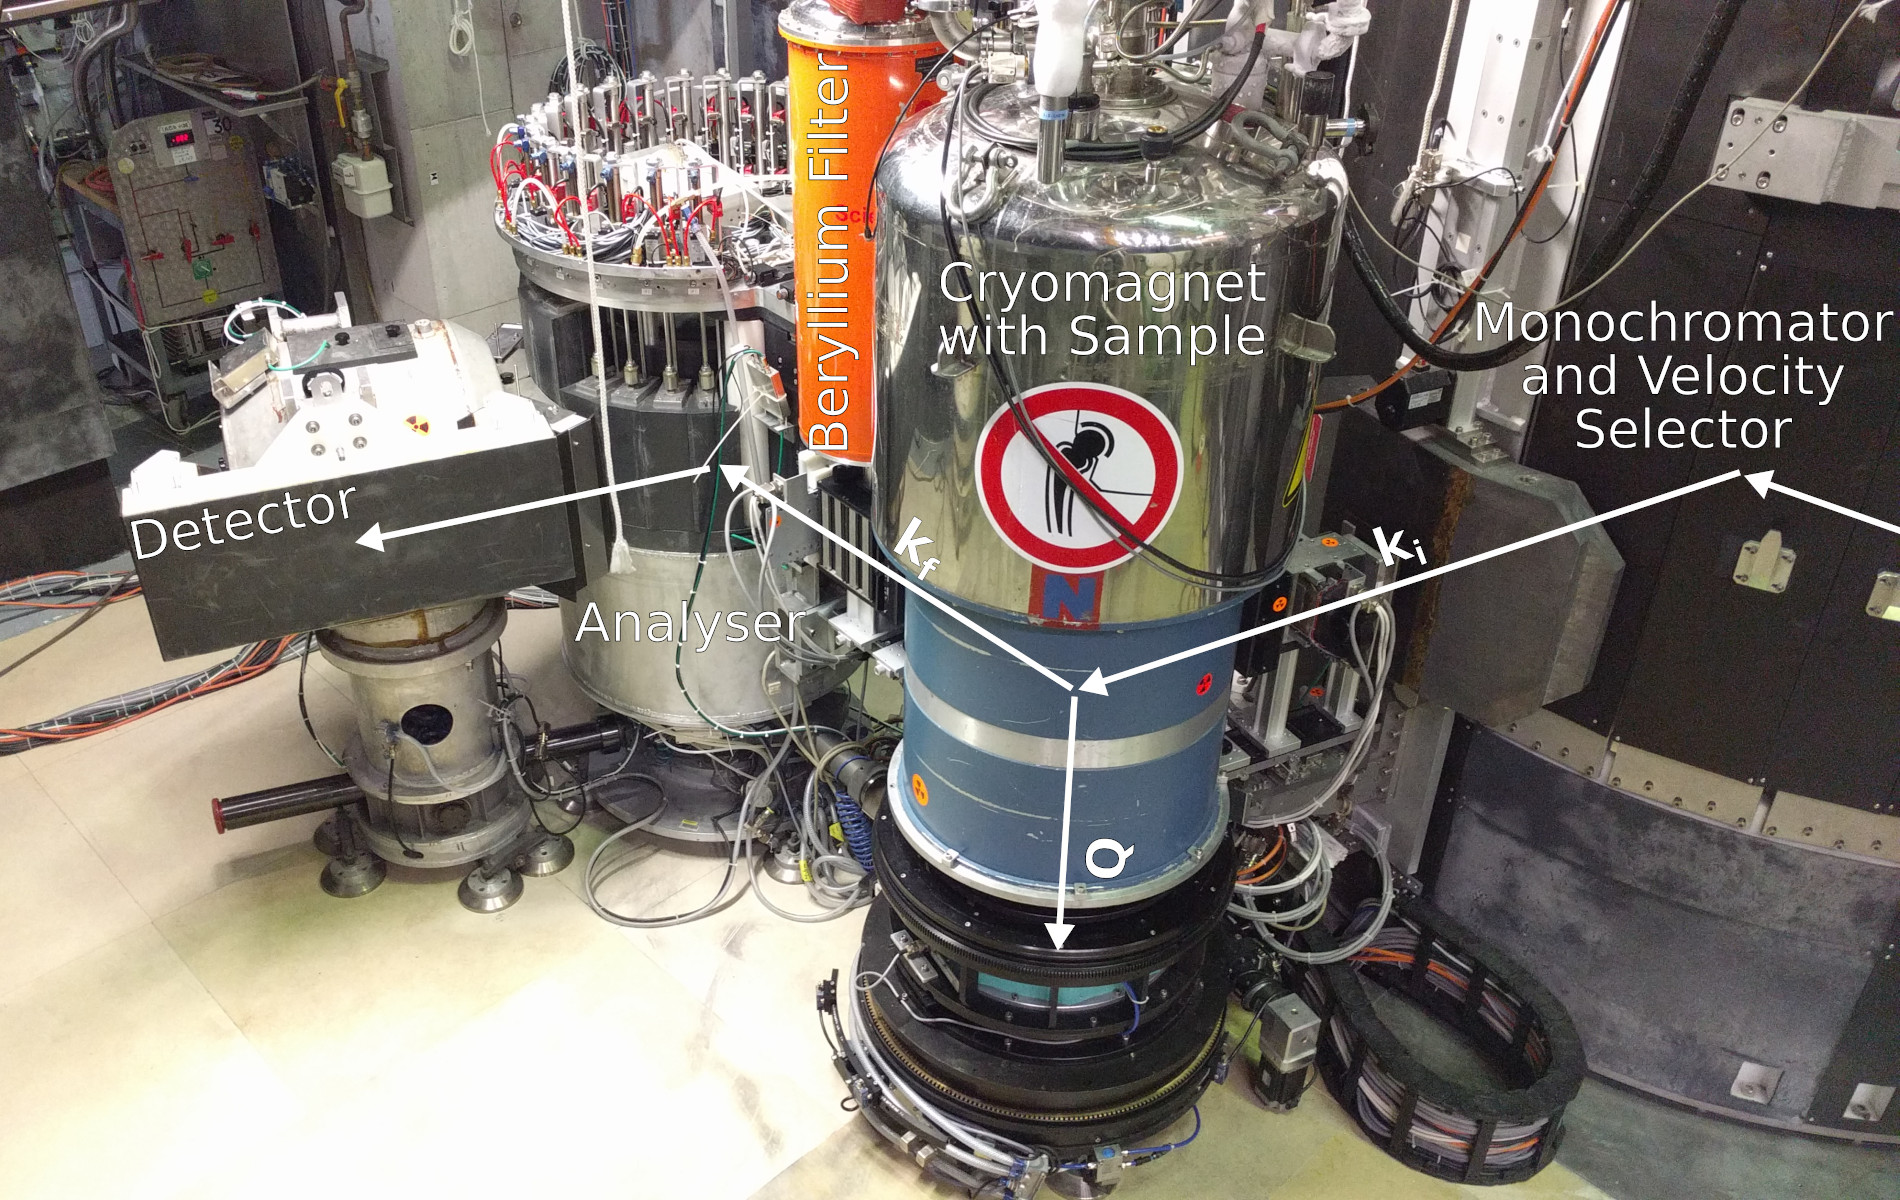
\includegraphics[width=0.75\textwidth]{figures/thales.jpg}
	\caption{The triple-axis spectrometer ThALES \cite{thales} at the Institut Laue-Langevin in Grenoble, France. The neutron path from the rector to the detector is marked as white arrows. The momentum transfer, $\hbar \bm{Q}$, is also shown. This picture is reproduced from \cite{skxpaper}.}
	\label{fig:thales}
\end{figure*}



\section{Autonomous experiments \label{sec:autonomous}}

Up until the end of 2019, TAS experiments usually required external scientists to stay at the research reactor for typically one week and conduct the experiment together with the instrument's responsible scientists. Specifically at the Institut Laue-Langevin (ILL) there had already been attempts (e.g. \cite{Song2020}) of the instrument control and scientific computing groups to convince the instrument scientists of the benefits of instrumentation with full- or semi-autonomous as well as remote control. Nevertheless, the impact had been limited.

The situation changed significantly with the Covid-19 pandemic. Receiving visiting scientists has not possible anymore, or only to a very limited degree. Instead, remote experimentation and instrument control has become the new norm. Users now connect to a web interface from which the experiment can be planned and data can be analysed~\footnote{\url{https://visa.ill.eu}}. Discussions with instrument scientists take place via web-cams that have been installed at every instrument.

At the same time, the idea to automate manual tasks at instruments using algorithms and AI has gained significant traction, with first autonomous experiments being attempted~\footnote{\url{https://www.ill.eu/news-press-events/news/scientific-news/machine-learning-at-ill-first-autonomous-steps-of-the-neutron-spectrometer-thales}}.
As part of the current drive towards autonomous experimentation at the ILL, the goal of the present work is the design and implementation of a software tool which enable an automatic path finding for TAS instruments. Automatic path finding is necessary for the instrument to circumvent obstacles in its path. Currently, this task has to be performed by the instrument scientists before each new scan series in a time-consuming fashion. The current approach requires the instrument to be  driven along the programmed scan path, but without measuring and with the neutron beam from the reactor closed. The instrument scientist has to stay in the instrument space and watch the instrument as it moves to every scan position. A manual stop has to be initiated when the instrument would collide with a wall or with itself or when the rotation of one of the axes would pull out a cable or tube.

In the next chapter, we will introduce the coordinate systems used in crystallography and at TAS instruments.
